\begin{pa} \label{PA:11.7} Consider a solid piece granite in the shape of a box $B = \{(x,y,z) : 0 \leq x \leq 4, 0 \leq y \leq 6, 0 \leq z \leq 8\}$, whose density varies from point to point. Let $\delta(x, y, z)$ represent the mass density of the piece of granite at point $(x,y,z)$ in kilograms per cubic meter (so we are measuring $x$, $y$, and $z$ in meters). Our goal is to find the mass of this solid. 

Recall that if the density was constant, we could find the mass by multiplying the density and volume;  since the density varies from point to point, we will use the approach we did with two-variable lamina problems, and slice the solid into small pieces on which the density is roughly constant.

Partition the interval $[0,4]$ into 2 subintervals of equal length, the interval $[0,6]$ into 3 subintervals of equal length, and the interval $[0,8]$ into 2 subintervals of equal length. This partitions the box $B$ into sub-boxes as shown in Figure \ref{F:11.7.Box_domain}.
\begin{figure}[h]
\begin{center}
%\resizebox{!}{2.0in}{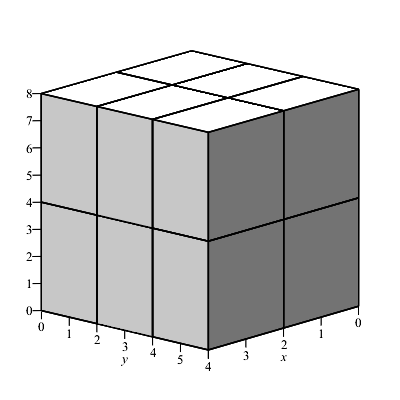
\includegraphics[trim=0cm 1cm 0cm 1cm, clip]{11_7_Box_domain}}
  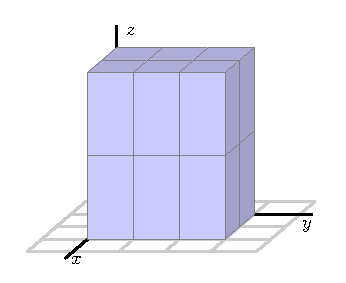
\includegraphics{figures/fig_11_7_preview.eps}
\end{center}
\caption{A partitioned three-dimensional domain.}
\label{F:11.7.Box_domain}
\end{figure}
%crop graphics in animate trim=<left> <bottom> <right> <top>, clip with includegraphics
    \ba
    \item Let $0=x_0 < x_1 < x_2=4$ be the endpoints of the subintervals of $[0,4]$ after partitioning. Draw a picture of Figure \ref{F:11.7.Box_domain} and label these endpoints on your drawing. Do likewise with $0=y_0 < y_1 < y_2 < y_3=6$ and $0=z_0 < z_1 < z_2=8$
    
    What is the length $\Delta x$ of each subinterval $[x_{i-1},x_i]$ for $i$ from 1 to 2?  the length of $\Delta y$?  of $\Delta z$?

	\item The partitions of the intervals $[0,4]$, $[0,6]$ and $[0,8]$ partition the box $B$ into sub-boxes. How many sub-boxes are there? What is volume $\Delta V$ of each sub-box?
	

	
	\item Let $B_{ijk}$ denote the sub-box $[x_{i-1},x_i] \times [y_{j-1},y_j] \times [z_{k-1}, z_k]$.
		%. Appropriately label each visible sub-box in your drawing of Figure \ref{F:11.7.Box_domain} according to this labeling scheme.
	Say that we choose a point $(x_{ijk}^*, y_{ijk}^*, z_{ijk}^*)$ in the $i,j,k$th sub-box for each possible combination of $i,j,k$.  What is the meaning of $\delta(x_{ijk}^*, y_{ijk}^*, z_{ijk}^*)$?  What physical quantity will $\delta(x_{ijk}^*, y_{ijk}^*, z_{ijk}^*) \Delta V$ approximate?
	

    \item What final step(s) would it take to determine the exact mass of the piece of granite?


\ea
\end{pa} 

\begin{activitySolution}

    \ba
    \item We have $x_0=0$, $x_1=2$, and $x_2=4$;  $y_0=0$, $y_1=2$, $y_2=4$, and $y_3=6$; and $z_0=0$, $z_1=4$, and $z_2=8$. This gives us $\Delta x = \frac{4-0}{2} = 2$, $\Delta y = \frac{6-0}{3} = 2$, and $\Delta z = \frac{8-0}{2} = 4$.  These points are labeled in figure below.

%\begin{figure}[h]
\begin{center}
\resizebox{!}{2.0in}{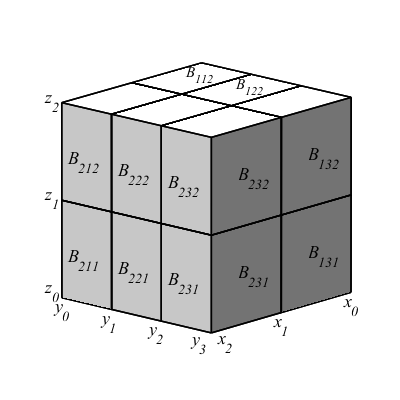
\includegraphics{figures/fig_11_7_Box_domain_PA_labeled.png}}
\end{center}
%\caption{A partitioned and labeled three-dimensional domain.}
%\label{F:11.7.Box_domain_PA_labeled}
%\end{figure}


	\item Since we partition the interval $[0,4]$ into 2 subintervals, the interval $[0,6]$ into 3 subintervals, and the interval $[0,8]$ into 2 subintervals, there are $(2)(3)(2) = 12$ sub-boxes of $B$.  Each sub-box has volume $\Delta x \ \Delta y \ \Delta z = (2)(2)(4) = 16$.

	
	\item The visible sub-boxes are labeled in the figure. Notice that we cannot see boxes
\[B_{111} = [x_0,x_1] \times [y_0, y_1] \times [z_0,z_1] \ \ \text{ and } \ \ B_{121} = [x_0,x_1] \times [y_1, y_2] \times [z_0,z_1].\]

If we consider the mass of the solid in sub-box $B_{ijk}$ as a constant $\delta(x_{ijk}^*, y_{ijk}^*, z_{ijk}^*)$ in kilograms per cubic meter, then the product $\delta(x_{ijk}^*, y_{ijk}^*, z_{ijk}^*) \Delta V$ will approximate the mass of the solid on sub-box $B_{ijk}$.


    \item To determine the mass of our solid, we sum the approximations of the masses on each sub-box and the take the limit as $\Delta x$, $\Delta y$, and $\Delta z$ go to 0. Thus, the mass of our solid is
\[\lim_{\substack{\Delta x \to 0 \\ \Delta y \to 0 \\ \Delta z \to 0}} \sum_{i=1}^m \sum_{j=1}^n \sum_{k=1}^l \delta(x_{ijk}^*, y_{ijk}^*, z_{ijk}^*) \Delta V.\]


\ea


\end{activitySolution}

\afterpa 